
\documentclass[
	% -- opções da classe memoir --
	12pt,				% tamanho da fonte
	oneside,			% para impressão em verso e anverso. Oposto a oneside
	a4paper,			% tamanho do papel. 
	brazil				% o último idioma é o principal do documento
	]{abntex2}

% ---
% Pacotes básicos 
% ---
\usepackage{pdflscape}
\usepackage{xcolor, listings}
\usepackage{fontspec}
\usepackage{longtable}
\setmainfont{Arial}
\usepackage[top=2cm, bottom=2cm, left=2cm, right=2cm]{geometry}
\usepackage[utf8]{inputenc}		% Codificacao do documento (conversão automática dos acentos)
\usepackage{indentfirst}		% Indenta o primeiro parágrafo de cada seção.
\usepackage{color}				% Controle das cores
\usepackage{graphicx}			% Inclusão de gráficos
\usepackage{microtype} 			% para melhorias de justificação
\usepackage{multicol}			% multiplas colunas no texto
\usepackage{graphicx,url}
\usepackage{float}
\usepackage{slashbox}
% ---
\lstset{language=SQL,
		keywordstyle=\color{blue},
           showspaces=false,
           basicstyle=\ttfamily,
           numbers=left,
           numberstyle=\tiny,
           commentstyle=\color{gray}
}

% ---
% Pacotes de citações
% ---
\usepackage[brazilian]{backref}	 % Paginas com as citações na bibl
\usepackage[alf]{abntex2cite}	% Citações padrão ABNT
\usepackage{indentfirst}
% --- 
% CONFIGURAÇÕES DE PACOTES
% --- 

% ---
% Configurações do pacote backref
% Usado sem a opção hyperpageref de backref
\renewcommand{\backrefpagesname}{Citado na(s) página(s):~}
% Texto padrão antes do número das páginas
\renewcommand{\backref}{}
% Define os textos da citação
\renewcommand*{\backrefalt}[4]{
	}%
% ---

% ---
% Informações de dados para CAPA e FOLHA DE ROSTO

% ---


% ---
% Configurações de aparência do PDF final

% alterando o aspecto da cor azul
\definecolor{blue}{RGB}{41,5,195}

% informações do PDF
\makeatletter
\hypersetup{
     	%pagebackref=true,
		pdftitle={\@title}, 
		pdfauthor={\@author},
    	pdfsubject={\imprimirpreambulo},
	    pdfcreator={LaTeX with abnTeX2},
		colorlinks=true,       		% false: boxed links; true: colored links
    	linkcolor=black,          	% color of internal links
    	citecolor=black,        		% color of links to bibliography
    	filecolor=magenta,      		% color of file links
		urlcolor=black,
		bookmarksdepth=4
}
\makeatother
% --- 

% --- 
% Espaçamentos entre linhas e parágrafos 
% --- 

% O tamanho do parágrafo é dado por:
\setlength{\parindent}{1.3cm}

% Controle do espaçamento entre um parágrafo e outro:
\setlength{\parskip}{0.2cm}  % tente também \onelineskip

% ---
% compila o indice
% ---
\makeindex
% ---

% ----
% Início do documento
% ----
\begin{document}

% Seleciona o idioma do documento (conforme pacotes do babel)
%\selectlanguage{english}
\selectlanguage{brazil}

% Retira espaço extra obsoleto entre as frases.
\frenchspacing 

% ----------------------------------------------------------
% ELEMENTOS PRÉ-TEXTUAIS
% ----------------------------------------------------------
% \pretextual



% ---
% Capa
% ---
%%%%%%%%%%%%%%%%   CAPA   %%%%%%%%%%%%%%%%%%%%%%      
%\begin{document} 



%\begin{titlepage}
\begin{center}

\begin{figure}[!htb]
%\centering

\includegraphics[width=1.1\textwidth]{USFCAR_-_logo.jpg}\

\end{figure}


\vspace{80pt}
\LARGE{\textbf{Bacharelado Ciência da Computação}}\\
\LARGE{Trabalho Integrado - Fase Intermediária}\\
\LARGE{ Tema 2}

\vspace{50pt}
\textbf{\Huge{}}

\end{center}
	
\begin{flushleft}
		
\begin{center}
{\Large 	Grupo 5\\
			 Aléssia Melo - 620289\\
			 Caio Henrique Giacomelli - 620297\\
  			 Gabriela Ramos - 620360\\
  			 Matheus Augusto Thomaz - 620599\\}
\end{center}
        
\vspace{70pt}

 \begin{center}

{\large { 01/06/2017 \\Bancos de Dados, Engenharia de Software II e WEB } \\
Profª Drª Sahudy Montenegro González\\
Profª Drª Luciana Zaina \\
Profº Drº Alexandre Álvaro} 
                    
\end{center}
        
\end{flushleft}	
  
%\end{titlepage}



% ---


% ---
% inserir o sumario
% ---
\pdfbookmark[0]{\contentsname}{toc}
\tableofcontents*
\cleardoublepage
% ---



% ----------------------------------------------------------
% ELEMENTOS TEXTUAIS
% ----------------------------------------------------------
\textual

% ----------------------------------------------------------
% Introdução (exemplo de capítulo sem numeração, mas presente no Sumário)
% ----------------------------------------------------------

% ----------------------------------------------------------



% ----------------------------------------------------------
% Apresentamos o texto
% ----------------------------------------------------------
\chapter{Especificação de Consultas SQL}
\section{Objetivo}
	Neste documento será descrito o processo de análise, normalização, indexação e otimização do banco de dados, tendo como objetivo responder questões centrais sobre decisões tomadas em relação ao processo de implementação do banco de dados referente a aplicação a ser desenvolvida.
    
    
   A aplicação possibilitará buscas avançadas de atores, que incluem o nome, intervalo de anos ou ano específico de filmes em que trabalhou, sexo e nome do personagem e também em quais filmes o ator X e o ator Y trabalharam juntos. 
   
   
   Além disso, constam neste documento o script contendo todos os códigos em SQL utilizados para a criação e manipulação do banco de dados, separados conforme os tópicos abrangidos nas seções e capítulos subsequentes. O script final será entregue em anexo no fim deste documento.
   
\section{Descrição das Consultas}
O sistema a ser desenvolvido será uma aplicação Web capaz de realizar consultas relacionadas a base de dados do IMBb, para isso, também contará com um sistema de paginação para possibilitar a visualização da grande massa de dados que serão retornados. Portanto, o sistema será composto por duas consultas principais:
 
\begin{itemize}

\item \textbf{Consulta 1:} trata-se de uma busca avançada de atores, que incluem o nome, intervalo de anos ou ano específico de filmes em que trabalhou, sexo e nome do personagem. Tal consulta será decomposta em:
\begin{itemize}
\item\textit{ Subconsulta 1:} Consulta de atores por sexo, nome relativo do personagem e ano específico em que estes trabalharam;
\item \textit{Subconsulta 2:} Consulta de atores por nome e intervalo de anos;
\end{itemize}
\item \textbf{Consulta 2:} trata-se de uma busca simples que correlaciona dois atores e retorna oa filmes em que estes trabalharam juntos.
\end{itemize}

Todas as consultas citadas retornarão algumas informações relacionadas aos atores, podendo conter título e ano do filme em que contracenaram, nome e sexo do ator, assim como o nome do personagem que este realizou. Outrossim, a consulta 2 será ordenada lexicograficamente pelos nomes dos atores

\section{Consulta 1}

\subsection{Subconsulta 1}
A primeira subconsulta tem como objetivo retornar o sexo, nome e personagem, assim como seus filmes e o ano do filme em que o ator atuou. Para isto, toma três parâmetros em consideração, o sexo do ator, o ano e o nome do personagem que o ator interpretou.

Para realizar esta consulta, realizamos um \textit{SELECT} nos retornos desejados, e unimos as três tabelas que possuímos em nosso banco, sempre utlizando uma condição relacionada ao parâmetro da consulta. 

É importante enfatizar a utilização da cláusula \textit{LIKE} com os operadores \textit{\%}, utilizada para buscas relativas. Esta será nossa única consulta que possui tal funcionalidade. Segue abaixo o código desta subconsulta.
\\

\begin{lstlisting}
SELECT title, mvyear, actorname, sex, as_character
  FROM (SELECT * FROM movie WHERE mvyear = <year>) a 
  
  INNER JOIN movie_actor b 
  ON (b.movieid = a.movieid AND b.as_character 
  LIKE <%character_name%> )
  
  INNER JOIN actor c ON b.actorid = c.actorid 
  AND sex = <sex>

\end{lstlisting}


\subsection{Subconsulta 2}
A segunda subconsulta, recebe como parâmetros o nome do ator e o intervalo de anos em que trabalhou, e possui os mesmos retornos que a subconsulta 1.

Para realizar a consulta, selecionamos todas as informações dos atores, excluindo os não referenciados pelo parâmetro, e concluímos com dois \textit{INNERS JOINS} com \textit{movie\_actor} e movie, sendo este último adicionado um \textit{AND} para verificar o intervalo de anos. Para melhor visualização, abaixo está o código desta subconsulta.


\begin{lstlisting}
SELECT actorname, sex, as_character, title, mvyear
  FROM (SELECT * FROM actor 
  WHERE actorname LIKE <actor_name> )a
  
  INNER JOIN movie_actor b ON (a.actorid = b.actorid)
  INNER JOIN movie c 
  ON (b.movieid = c.movieid 
  AND (c.mvyear >= <year_1> AND c.mvyear <= <year_2>))

\end{lstlisting}


\section{Consulta 2}

Esta busca retornará os filmes em que dois atores (referenciados na consulta por <actor\_name\_1> e <actor\_name\_2>) trabalharam em conjunto. É importante notar que a busca será apenas absoluta.

Para realizar a consulta, utilizamos a operação \textit{INTERSECT} entre duas tabelas que eram compostas por um \textit{INNER JOIN} entre \textit{actor} e \textit{movie\_actor}, já excluindo os nomes de atores diferentes dos parâmetros relacionados. Após isto, realizamos mais uma junção com a tabela \textit{movie} para possuirmos os dados convenientes ao retorno da consulta. 

Informações sobre a decisão da ordem de seleção de informações serão dadas no capítulo 3. Segue abaixo o código da consulta:
\\
\begin{lstlisting}
SELECT * FROM ((SELECT ma.movieid
  FROM (
  SELECT * FROM actor a WHERE a.actorname = <actor_name_1> ) c
  INNER JOIN  movie_actor ma ON ma.actorid = c.actorid ) 
    
INTERSECT 

(SELECT ma.movieid
  FROM (
  SELECT * FROM actor a WHERE a.actorname = <actor_name_2>) c
  INNER JOIN  movie_actor ma ON ma.actorid = c.actorid)) movies 
  INNER JOIN movie m ON movies.movieid = m.movieid ORDER BY m.title

\end{lstlisting}


\chapter{Normalização do Banco de Dados}

Inicialmente, o banco de dados fornecido contendo dados do IMBD, era composto por apenas duas tabelas: \textit{movies} e \textit{directorsmovies}. Estas não continham chaves primárias, nem chaves secundárias e apresentavam as seguintes colunas: 

\begin{lstlisting}
MOVIES
(
  movieid integer,
  title character varying(400),
  mvyear character varying(100),
  actorid integer,
  actorname character varying(250),
  sex character(1),
  as_character character varying(1000),
  languages character varying(1000),
  genres character varying(100)
)
\end{lstlisting}

\begin{lstlisting}
DIRECTORSMOVIES
(
  movieid integer,
  directorid integer,
  dname character varying(500),
  addition character varying(1000)
)
\end{lstlisting}

Devido a descrição do problema, especificado na seção 1.2, o grupo optou por eliminar colunas que não eram relevantes ao domínio do problema. Assim, para que o banco de dados seguisse a 3º forma normal, foi necessário realizar a separação de \textit{movies} em três tabelas, como apresentado no esquema abaixo:
\newpage

\begin{figure}
\centering
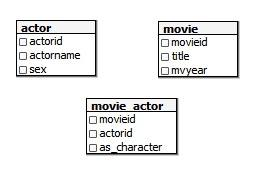
\includegraphics{modeloBanco.jpg}
\caption{Modelo simplificado das tabelas do Banco de Dados Final}

\end{figure}

Após a exclusão de colunas desnecessárias, considerando o escopo do tema, foram criadas as duas tabelas principais \textit{movie} e \textit{actor}, onde suas estruturas podem ser verificadas no esquema abaixo.
\\
\begin{lstlisting}
CREATE TABLE public.movie
(
  movieid integer,
  title character varying(400),
  mvyear character varying(100)

CONSTRAINT movie_pkey PRIMARY KEY (movieid)
)

CREATE TABLE public.actor
(
  actorid integer,
  actorname character varying(250),
  sex character(1),

CONSTRAINT actor_pkey PRIMARY KEY (actorid)
)
\end{lstlisting}

Com relação aos personagens, pode-se notar que é um dado do tipo \textit{n:n}. O banco fornecido apresentava os dados na forma multivalorada, onde (na maior parte dos casos) os vários personagens que um ator interpretou em um mesmo filme seguia o seguinte formato: 

\begin{center}
\textbf{[personagem 1>/<personagem 2>/.../<personagem n]}
\newline
\end{center}


Constatando isto, foi possível separar tais dados, por meio da função \textbf{regexp\_split\_to\_ table}, criando assim uma nova tabela chamada \textit{movie\_actor} onde sua estrutura está detalhada no script abaixo, bem como a função utilizada. 
\\

\begin{lstlisting}
CREATE TABLE public.movie_actor
(
  movieid integer,
  actorid integer,
  as_character character varying(1000),

CONSTRAINT movieactorid_pkey PRIMARY KEY (movieid, actorid)

INSERT INTO movie_actor SELECT DISTINCT
    movieid,actorid, 
    regexp_split_to_table(as_character, E'/') AS split_character
FROM temporaria
)
\end{lstlisting}

Alguns pontos da estrutura dos dados do banco fornecido são importantes de serem destacados:
\begin{itemize}

\item O banco contém diversas inconsistências de dados, tais como, símbolos ",", "<", ">", "/"  em diversas colunas, dados não relevantes para o escopo junto a dados que estão sendo utilizados (Ex:"[ADA Jeffrey Brandau]  <12>", o dado "<12>"  é irrelevante), colunas com dados vazios (com caractere de espaço apenas), colunas com dados do tipo "?????", além de diversas tuplas que não representam filmes (sem conter nenhuma indicação do tipo).

\item Todos os dados são do tipo texto (character varying).

\end{itemize}

As inconsistências descritas acima acarretarão em um visualização pouco agradável dos dados e em uma certa lentidão na busca, pois o tipo de dados de todos os campos (com exceção dos IDs) é texto, e é sabido que, uma busca por texto é muito mais lenta do que uma consulta por meio de números, e uma vez que há caracteres "estranhos"  não se consegue alterar o tipo de dado de \textit{character} para \textit{integer} no campo de ano, por exemplo. 

Vale salientar que tais inconsistências não serão corrigidas, pois o banco é extenso e este não é o objetivo do presente trabalho.

\newpage
\chapter{Técnicas de Acesso Eficiente ao BD}

\section{Indexação}
Nesta seção serão apresentadas as estruturas de indexação utilizadas neste trabalho, quais os resultados obtidos por trás dos índices e quais colunas julgamos necessárias possuirmos índices para otimizarmos as consultas.

Abaixo segue uma breve descrição de cada índice criado:

Índice do tipo hash na coluna de actorid da tabela \textit{Actor}, aplicado na subconsulta 1.

\begin{lstlisting}
CREATE INDEX hash_actorid
  ON public.actor
  USING hash
  (actorid);
\end{lstlisting}

Índice do tipo BTree na coluna de actorname da tabela \textit{Actor}, aplicado na consulta 2 e na subconsulta 2.
\begin{lstlisting}
CREATE INDEX index_name_actor
  ON public.actor
  USING btree
  (actorname COLLATE pg_catalog."default");
\end{lstlisting}

Índice do tipo BTree na coluna de movieid da tabela \textit{Movie}, aplicado na consulta 2 e na subconsulta 2.
\begin{lstlisting}
CREATE UNIQUE INDEX movieid_index
  ON public.movie
  USING btree
  (movieid);
\end{lstlisting}

Índice do tipo BTree na coluna de mvyear da tabela \textit{Movie}, aplicado na subconsulta 1.
\begin{lstlisting}
CREATE INDEX mvyear_index
  ON public.movie
  USING btree
  (mvyear COLLATE pg_catalog."default");
\end{lstlisting}

\newpage

Índice do tipo gin (Generallizated Inverted Index) na coluna de \textit{as\_character} da tabela \textit{movie\_actor}, aplicado na subconsulta 1.
\begin{lstlisting}
CREATE INDEX chatacter_index_gin
  ON public.movie_actor
  USING gin
  (as_character COLLATE pg_catalog."default" gin_trgm_ops);
\end{lstlisting}

Índice do tipo BTree na coluna de actorid da tabela \textit{movie\_actor}, aplicado na consulta 2 e na subconsulta 2.
\begin{lstlisting}
CREATE INDEX idx_actor
  ON public.movie_actor
  USING btree
  (actorid);
\end{lstlisting}
\newpage

\section{Otimização}

\subsection{Subconsulta 1}
\begin{center}
\begin{tabular}{|l|*{4}{c|}}\hline
\makebox[2em]{\textbf{}}&\makebox[10em]{\textbf{Subconsulta 1 Inicial}}&\makebox[13em]{\textbf{Subconsulta 1 Otimizada}}&\makebox[10em]{\textbf{Diferença (\%)}}\\\hline\hline

T.E. & 12.3 segundos & 22.1 segundos & -80\\\hline
T.E. & 12.5 segundos & 22.9 segundos & -83,2 \\\hline
T.E. & 13.0 segundos & 23.5 segundos & -80,7\\\hline
T.E. & 14.9 segundos & 23.0 segundos & -54,4 \\\hline
T.E. & 15.9 segundos & 23.2 segundos & -45,9\\\hline
Média & 13.72 segundos & 22.94 segundos & -67,2\\\hline
\end{tabular}
\end{center}

Inicialmente foi elaborada uma consulta com os conhecimentos básicos de BD, o tempo de retorno, como é possível evidenciar pela tabela, foi razoável, com uma média de 13.72 segundos. Como o projeto visa, dentre outras coisas, o aprendizado da otimização de consultas, o conceito de subdivisão em queries foi aplicado, bem como a criação de índices.

Nesta consulta foram criados e utilizados os índices de hash\_actorid, mvyear\_index e chatacter\_index\_gin. Hash\_actorid, mvyear\_index foram criados, pois são usados nas cláusulas \textit{where} e \textit{inner join}, que nada mais são do que os campos em que a consulta será efetivamente aplicada. 

Já o chatacter\_index\_gin é um índice otimizado para \textit{selects}, especialista em comparação de strings. Ele é ideal para o sub select desta consulta, pois há uma busca por texto de modo relativo, por meio da cláusula \textit{like}. Esta escolha foi feita, pois o gerenciador de banco de dados não utiliza índices ao identificar uma busca relativa, e acaba realizando uma busca sequencial. (Pode-se constatar esta afirmação no plano de consulta indicado pela figura 2).

Uma das estratégias de otimização utilizadas foi a quebra da consulta não otimizada em sub queries, visando selecionar primeiramente as sub-relações que continham menos tuplas, reduzindo assim o número de combinações. Pode-se observar este caso claramente na inversão da seleção do sexo com o ano, no código completo em anexo.

Porém, como é possível notar por meio da observação da tabela, o tempo de retorno da consulta otimizada foi cerca de 23 segundos, em média. Levando 67\% a mais de tempo se comparado à consulta não otimizada. 

Isto se deu pelo fato de que na consulta otimizada, apesar de estar utilizando o índice gin, também é realizada uma busca Bitmap. Ao fazer um index scan (antes de fazer o Bitmap), o otimizador visita o índice para encontrar as localizações das linhas que correspondem à condição do índice e, em seguida, estas linhas são efetivamente obtidas. Obter as linhas separadamente é mais custoso do que lê-las sequencialmente, mas como nem sempre nem todas as páginas da tabela devem ser visitadas, isso se torna mais barato do que uma varredura sequencial. 


\newpage

\begin{landscape}
\begin{figure}
\centering
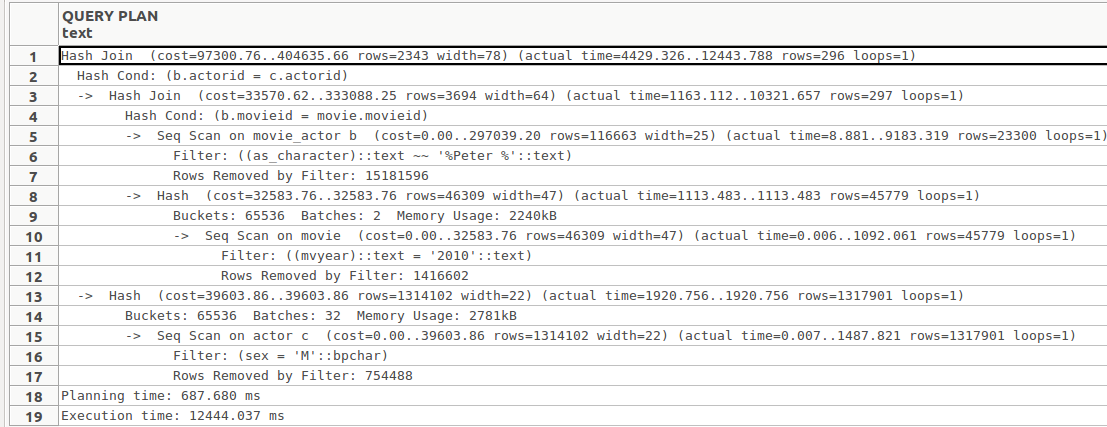
\includegraphics[scale = 0.7]{consulta1_naootimizada_sub1.png}
\caption{Consulta 1 - sub. 1 -  Não otimizada}
\end{figure}
\begin{figure}
\centering
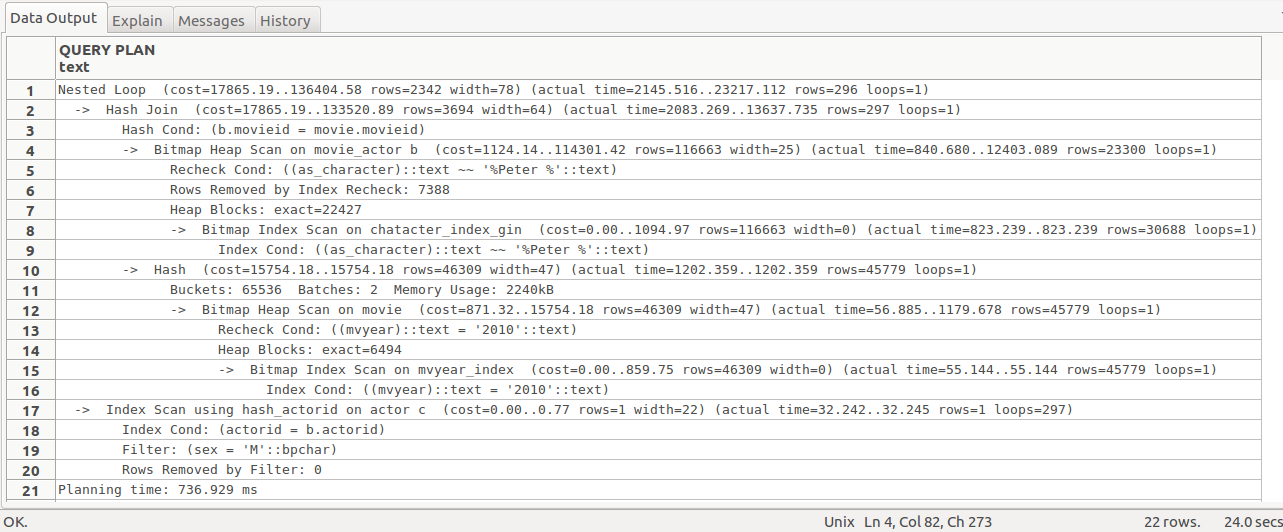
\includegraphics[scale = 0.7]{Consulta1_opt_sub1.png}
\caption{Consulta 1 - sub. 1 - Otimizada}
\end{figure}
\end{landscape}

\newpage


\subsection{Subconsulta 2}

\begin{center}
\begin{tabular}{|l|*{4}{c|}}\hline
\makebox[2em]{\textbf{}}&\makebox[10em]{\textbf{Subconsulta 2 Inicial}}&\makebox[13em]{\textbf{Subconsulta 2 Otimizada}}&\makebox[10em]{\textbf{Diferença (\%)}}\\\hline\hline

T.E. & 12.7 segundos & 6.4 segundos & 49.6\\\hline
T.E. & 11.7 segundos & 6.7 segundos & 42.7\\\hline
T.E. & 11.6 segundos & 6.5 segundos & 44.0\\\hline
T.E. & 13.6 segundos & 6.6 segundos & 51.5\\\hline
T.E. & 11.4 segundos & 6.5 segundos & 43.0\\\hline
Média & 12.2 segundos & 6.54 segundos & 46.4\\\hline
\end{tabular}
\end{center}

\indent Para realizar a subconsulta 2, primeiramente foi implementada a consulta de forma não otimizada, na qual as tabelas foram unidas antes das cláusulas \textit{WHERE} serem efetuadas. Por esse motivo o valor de execução inicial da consulta difere moderadamente do tempo utilizado na consulta otimizada. Para um melhor entendimento dos dados retornados pela consulta, foi aplicada uma atualização nas tuplas cujo \textit{actorname} corresponde ao nome "Hathaway, Anne", que foi a atriz selecionada para exemplificação das buscas. 
\\\indent Após verificar o funcionamento dos índices e estudar o problema, foi constatado que a alteração da ordem das consultas bem como o uso de índices não utilizados anteriormente, poderiam melhorar o desempenho das consultas realizadas. Tais alterações seguem o conceito de otimização.
\\\indent O primeiro passo para otimização da consulta foi a inversão da ordem das consultas. Após analisar o banco, verificou-se que a tabela \textit{movie\_actor} era a tabela com maior quantidade de tuplas, e que para melhor desempenho era necessário filtrar ao máximo o número de tuplas antes de realizar a junção com a mesma. Para execução dessa modificação optou-se por realizar primeiramente a consulta que retorna os atores com o nome pré-selecionado, visto que tal ação eliminaria uma grande parte da junção com a tabela de maior custo.
\\\indent Já em relação ao uso de índices, utilizou-se de testes para avaliar o índice que melhoraria o tempo de resposta da consulta além da análise do plano de execução da consulta, onde se pode obter informações sobre o tipo de índice que a consulta melhor se adaptaria. Nesta consulta foram utilizados os índices \textit{actorname} na tabela \textit{actor}, \textit{actorid} na tabela \textit{movie\_actor} e por último \textit{movieid} na tabela \textit{movie}.
\\\indent Os parâmetros utilizados na consulta, como especificado em parte anteriormente, foram os seguintes:
\begin{itemize}
\item Actor: Hathaway, Anne
\item Year: 1990 - 2010
\end{itemize}\newpage

\newpage

\begin{landscape}
\begin{figure}
\centering
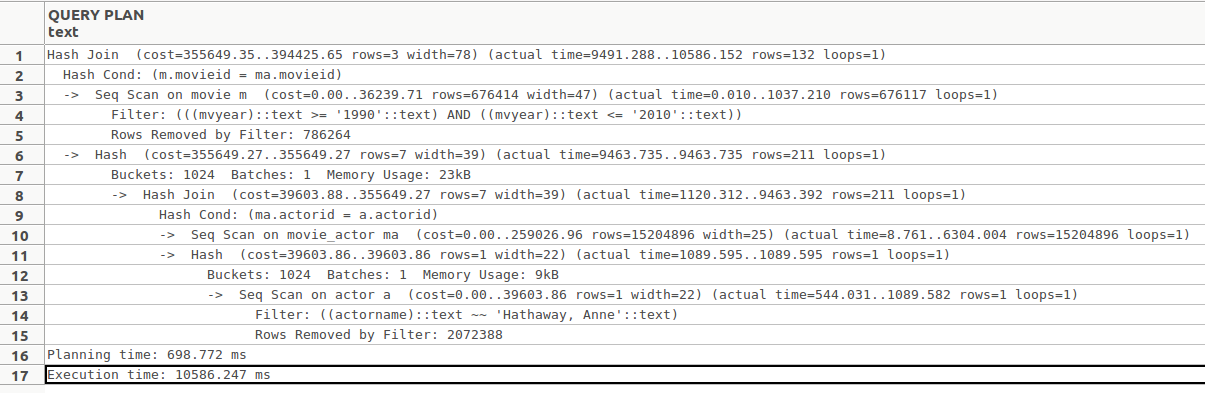
\includegraphics[scale = 0.7]{Consulta1_naootimizada_sub2.png}
\caption{Consulta 1 -sub.2 - Não Otimizada}
\end{figure}
\begin{figure}
\centering
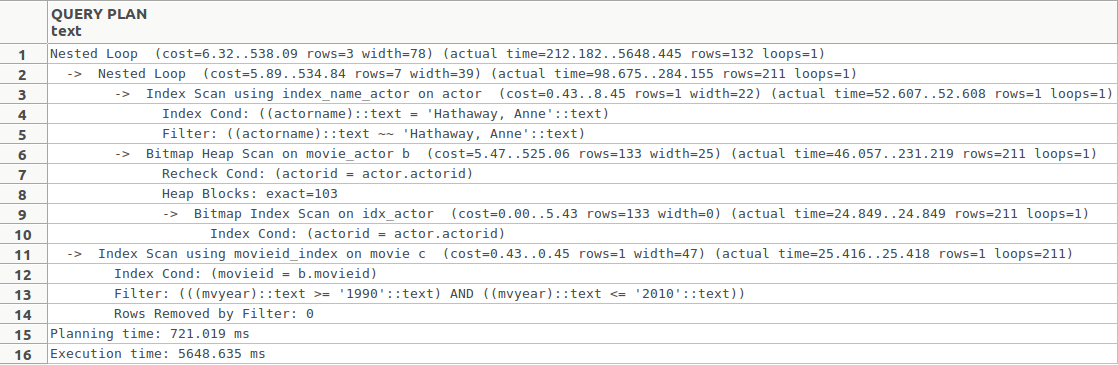
\includegraphics[scale = 0.7]{Consuta1_opt_sub2__1_.png}
\caption{Consulta 1 - sub.2 - Otimizada}
\end{figure}
\end{landscape}

\newpage

\indent A partir do plano de consulta acima pode-se notar que a consulta inicial não utilizava índice para a busca dos dados, realizando então uma busca sequêncial. O custo para a realização desta operação quando comparado ao custo da busca efetuada utilizando-se de índices é alto, como pode-se notar na Figura 4. Esse alto custo relacionado à busca sequencial pode ser notado quando analisamos a diferença entre o tempo de execução das consultas, observando a tabela de diferença percebemos que houve uma melhoria de 46\%, reafirmando assim a melhor eficiência na utilização dos índices. 

\subsection{Consulta 2}


\begin{center}
\begin{tabular}{|l|*{4}{c|}}\hline
\makebox[2em]{\textbf{}}&\makebox[10em]{\textbf{Consulta 2 Inicial}}&\makebox[13em]{\textbf{Consulta 2 Otimizada}}&\makebox[10em]{\textbf{Diferença (\%)}}\\\hline\hline


T.E. & 23.9 segundos & 2.6 segundos & 89.1 \\\hline
T.E. & 23.6 segundos & 2.7 segundos & 88.5  \\\hline
T.E. & 23.2 segundos & 2.7 segundos & 88.4  \\\hline
T.E. & 24.2 segundos & 2.8 segundos & 88.4  \\\hline
T.E. & 24.0 segundos & 3.3 segundos & 86.3 \\\hline
Média & 23.78 segundos & 2.82 segundos & 88.1\\\hline
\end{tabular}
\end{center}

Primeiramente, realizamos a consulta 2 apenas aplicando nossos conhecimentos, sem pensarmos em utilizações de índices ou otimizações, e a consulta era composta por um \textit{INTERSECT} entre duas tabelas que continham todos os filmes em que atores X e Y co-atuaram. Note, como explícito na tabela, o elevado tempo inicial para realizar a consulta, com uma média de 23.78 segundos.

Após análises, escolhemos os índices relacionados aos parâmetros de \textit{INNER JOINS} e cláusulas de \textit{WHERE} (Bem especificados na seção 3.1) e aplicamos algumas técnicas de otimização. Como um exemplo destas técnicas, encontrou-se a necessidade de afunilar a quantidade de tuplas antes de juntarmos as tabelas. Como solução a este problemas, realizamos a operação de \textit{INTERSECT} antes de realizarmos o \textit{INNER JOIN} com a tabela movies, como aponta o código na seção 1.4, e após esta estratégia, em média, a consulta aumentou sua performance em 88.1\%.

É importante apontar que os parâmetros utilizados para estes testes foram:

\begin{itemize}
\item Actor 1: 'Aniston, Jennifer'
\item Actor 2: 'Perry, Matthew'
\end{itemize}

Para que este teste fosse mais limpo e conciso, realizamos um update na tabela, alterando o nome 'Aniston, Jennifer (I)' para 'Aniston, Jennifer' e também o nome 'Perry, Matthew (I)' para 'Perry, Matthew', como mostra o código abaixo:
\\
\begin{lstlisting}
UPDATE actor SET actorname='Aniston, Jennifer'
WHERE actorname LIKE 'Aniston, Jennifer (I)'

UPDATE actor SET actorname='Perry, Matthew' 
WHERE actorname 
LIKE 'Perry, Matthew (I)'
\end{lstlisting}

\newpage

\begin{landscape}
\begin{figure}
\centering
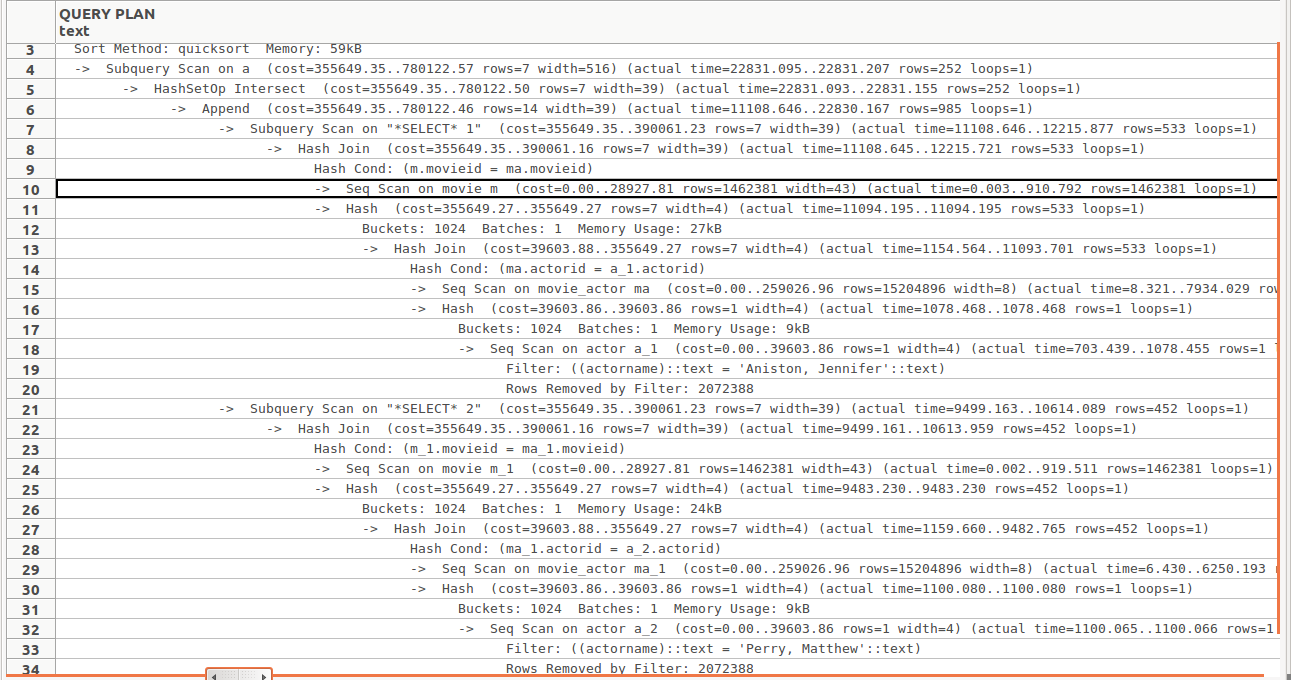
\includegraphics[scale = 0.7]{Consulta2_nao_otimizada.png}
\caption{Consulta 2 Não Otimizada}
\end{figure}
\begin{figure}
\centering
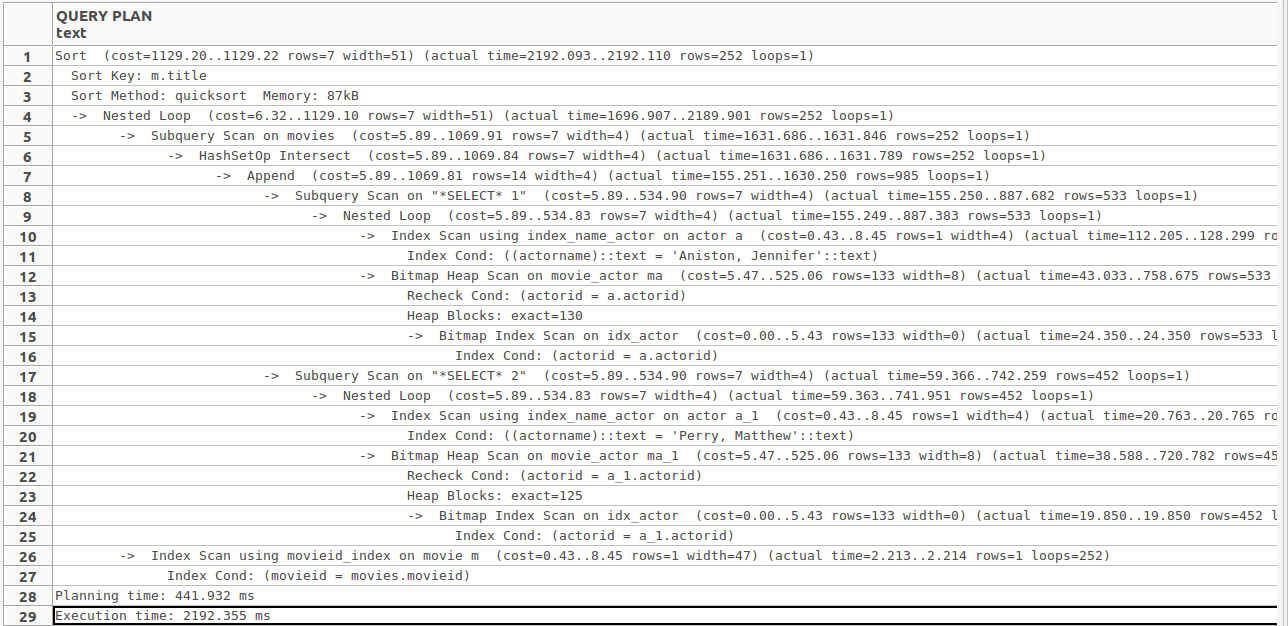
\includegraphics[scale = 0.7]{consulta2.png}
\caption{Consulta 2 Otimizada}
\end{figure}
\end{landscape}

Interpretando o plano de execução das consultas, é bem claro perceber que a consulta não otimizada utilizou \textit{SEQ SCANs} de custos altíssimos, que impactam diretamente na performance da consulta (Como exemplo, o \textit{SeqScan} sinalizado no plano da consulta). Isto acontece porque ainda não havia nenhum índice para a realização da mesma, e a busca sequencial foi necessária.

Já a imagem relacionada a consulta otimizada, utiliza os índices de name\_actor para ambas as cláusulas LIKE, assim como também utiliza o índice idx\_actor para o \textit{INNER JOIN}. O otimizador também seleciona o índice movieid\_index para realizar o último \textit{INNER JOIN}, nas etapas finais do plano de execução.

Percebe-se que o custo de uma busca sequencial é 50 vezes maior que o custo de um Bitmap Heap Scan, a operação mais custosa da consulta otimizada.


\newpage




\chapter{Anexos}

\begin{lstlisting}
-- Criação da tabela movie e inserção de dados
CREATE TABLE public.movie
(
  movieid integer,
  title character varying(400),
  mvyear character varying(100)

CONSTRAINT movie_pkey PRIMARY KEY (movieid)
)

INSERT INTO public.movie(movieid,title,mvyear)
     SELECT DISTINCT movieid, title, mvyear FROM public.movies
     
     
-- Criação da tabela actor e inserção de dados
CREATE TABLE public.actor
(
  actorid integer,
  actorname character varying(250),
  sex character(1),

CONSTRAINT actor_pkey PRIMARY KEY (actorid)
)

INSERT INTO public.actor(actorid,actorname,sex)
     SELECT DISTINCT actorid, actorname, sex FROM public.movies

-- Criação da tabela movie_actor e inserção de dados
CREATE TABLE public.movie_actor
(
  movieid integer,
  actorid integer,
  as_character character varying(1000),

CONSTRAINT movieactorid_pkey PRIMARY KEY (movieid, actorid)
)

ALTER TABLE movie_actor

  ADD CONSTRAINT actor_fkey FOREIGN KEY (actorid)
      REFERENCES public.actor (actorid) MATCH SIMPLE
      ON UPDATE NO ACTION ON DELETE NO ACTION,

  ADD CONSTRAINT movie_fkey FOREIGN KEY (movieid)
      REFERENCES public.movie (movieid) MATCH SIMPLE
      ON UPDATE NO ACTION ON DELETE NO ACTION
      
 INSERT INTO public.movie_actor(movieid,actorid,as_character)
     SELECT movieid,actorid,as_character FROM public.movies 

 INSERT INTO public.movie_actor(movieid,actorid,as_character)
     SELECT DISTINCT movieid, actorid,as_character FROM public.movies 

-- Split na coluna as_character, eliminando os espaços 
-- e separando os demais caracteres em tuplas diferentes
INSERT INTO movie_actor SELECT DISTINCT
    movieid,actorid, 
    regexp_split_to_table(as_character, E'/') AS split_character
FROM temporaria

-- Criação de índices
CREATE INDEX hash_actorid
  ON public.actor
  USING hash
  (actorid);

CREATE INDEX index_name_actor
  ON public.actor
  USING btree
  (actorname COLLATE pg_catalog."default");

CREATE UNIQUE INDEX movieid_index
  ON public.movie
  USING btree
  (movieid);

CREATE INDEX mvyear_index
  ON public.movie
  USING btree
  (mvyear COLLATE pg_catalog."default");

CREATE INDEX chatacter_index_gin
  ON public.movie_actor
  USING gin
  (as_character COLLATE pg_catalog."default" gin_trgm_ops);

CREATE INDEX idx_actor
  ON public.movie_actor
  USING btree
  (actorid);
  
-- Consulta 1

-- Subconsulta 1
SELECT title, mvyear, actorname, sex, as_character
 FROM (SELECT * FROM movie WHERE mvyear = '2010') a 
INNER JOIN movie_actor b ON (b.movieid=a.movieid 
AND b.as_character LIKE '%Peter %' )
INNER JOIN actor c ON b.actorid = c.actorid AND sex = 'M'

-- Subconsulta 2
EXPLAIN ANALYSE
SELECT * FROM (SELECT * FROM actor WHERE actorname 
LIKE 'Hathaway, Anne' )a 
INNER JOIN movie_actor b ON (a.actorid = b.actorid)
INNER JOIN movie c ON (b.movieid = c.movieid and(c.mvyear >= '1990' 
AND c.mvyear <= '2010' ))

-- Update nas colunas
UPDATE actor SET actorname='Hathaway, Anne' WHERE actorname 
LIKE 'Hathaway, Anne (I)'

UPDATE actor set actorname='Aniston, Jennifer' WHERE actorname 
LIKE 'Aniston, Jennifer (I)'

UPDATE actor set actorname='Perry, Matthew' WHERE actorname 
LIKE 'Perry, Matthew (I)'




-- Consulta 2
SELECT * FROM ((SELECT ma.movieid
   FROM (
   SELECT * FROM actor a
   WHERE a.actorname = 'Aniston, Jennifer') c
   INNER JOIN  movie_actor ma ON ma.actorid = c.actorid ) 
   INTERSECT 

   (SELECT ma.movieid
   FROM (
   SELECT * FROM actor a 
   WHERE a.actorname = 'Perry, Matthew') c
   INNER JOIN  movie_actor ma 
   ON ma.actorid = c.actorid)) movies INNER JOIN movie m 
   ON movies.movieid = m.movieid 
   ORDER BY m.title
   
-- Subconsulta 1 Não Otimizada

SELECT title, mvyear, actorname, sex, as_character
    FROM actor c INNER JOIN movie_actor b ON b.actorid = c.actorid
    AND sex = 'M'
    INNER JOIN (select * from movie where mvyear = '2010') a  
	ON (a.movieid =  b.movieid 
    AND b.as_character LIKE '%Peter %')
    
-- Subconsulta 2 Não Otimizada

SELECT title, mvyear, actorname, sex, as_character 
FROM actor a, movie_actor ma , movie m
WHERE ma.movieid = m.movieid AND ma.actorid = a.actorid
AND a.actorname like 'Hathaway, Anne' 
AND (m.mvyear >= '1990' AND m.mvyear <= '2010' )








-- Consulta 2 Não Otimizada

SELECT * FROM(SELECT m.title
	FROM actor a 
	INNER JOIN  movie_actor ma ON ma.actorid = a.actorid 
    INNER JOIN movie m  ON m.movieid = ma.movieid 
    WHERE a.actorname = 'Aniston, Jennifer'
 
	INTERSECT
        
SELECT m.title
	FROM actor a 
	INNER JOIN  movie_actor ma ON ma.actorid = a.actorid 
    INNER JOIN movie m  ON m.movieid = ma.movieid 
    WHERE a.actorname = 'Perry, Matthew') a ORDER BY a.title

\end{lstlisting}

% Referências bibliográficas
% ---------------------------------------------------------

\begin{thebibliography}{4}

\bibitem{Documentação PostgreSQL} "Documentação PostgreSQL.", https://www.postgresql.org/docs/.

\bibitem{Post GIS} "Post GIS", http://www.postgis.net.

\bibitem{Indíces PostgreSQL} "Índices PostgreSQL.", https://devcenter.heroku.com/articles/postgresql-indexes.


\bibitem{Indíces PostgreSQL} "Aulas de LabBD ministradas pela Professora Sahudy, UFSCar-S", https://ava.ead.ufscar.br/course/view.php?id=2576
\end{thebibliography}




%---------------------------------------------------------------------
% INDICE REMISSIVO
%---------------------------------------------------------------------
\phantompart
\printindex
%---------------------------------------------------------------------






\end{document}
